% Section 3 -- System design and methods, organised by the five stages of use (collect and clean; decide; review;
% tell the farmers; record what happened). Every number is a \kn{} macro from results/ (paper/numbers.py).
\section{System Design and Methods}
\label{sec:system}

\draftfor{Drafted by Claude from the built and tested system and the pre-registered protocol
(\texttt{layers/L3a\_forecasting/PREREGISTERED\_PROTOCOL.md}). The authors rewrite it in their own
words, redraw Fig.~\ref{fig:architecture} to match the five stages below, and check each statement
against the code before submission.}

KisanNiti is organised as the sequence in which an FPO manager uses it (Fig.~\ref{fig:architecture}):
(1)~farmer records, mandi prices and storage readings are collected and cleaned; (2)~a forecast, a
storage assessment and a fair allocation are turned into a proposed selling plan; (3)~the manager
reviews, edits and approves or rejects it; (4)~each farmer is told in their own language; and
(5)~replies and actual sales are recorded and compared with the plan. Five rules hold throughout.
Raw facts, derived values, system proposals, human decisions and what actually happened are stored
separately and never overwrite each other. Quantities and money are exact (grams and paise, never
floating point). Every FPO sees only its own data, enforced twice, in the query and in the database.
Every change is an append-only record with the person and request that made it. Every failure is
explicit: a missing contact, consent or language blocks a message with a stated reason instead of
being guessed.

\begin{figure}[t]
  \centering
  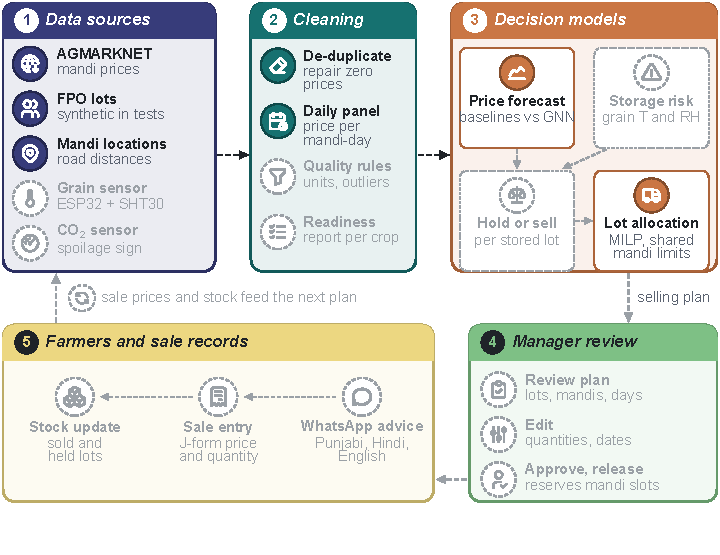
\includegraphics[width=\textwidth]{fig1_architecture.pdf}
  \caption{KisanNiti architecture. Data sources (1) are cleaned into a daily mandi price
  panel (2). Decision models (3) turn prices, storage readings and lot records into a selling
  plan that the FPO manager reviews (4). Farmers receive the approved plan on WhatsApp, and
  their recorded sales update stock for the next plan (5). MILP: mixed-integer linear program;
  GNN: graph neural network; RH: relative humidity.}
  \label{fig:architecture}
\end{figure}

\subsection{Stage 1: Data and Cleaning}
\label{sec:method-data}

Prices come from the AGMARKNET report \emph{Date Wise Prices for Specified Commodity}, downloaded
by hand for each month because the portal asks for a CAPTCHA. \kn{data_manifests} months of Paddy
(Basmati) for Punjab are filed with a manifest of checksums and row counts. A parser keeps every
line with its source file and position, so that each row of the cleaned table can be traced to the
line it came from. The \kn{data_manifests} monthly files hold \kn{data_rows_total} rows (\kn{data_rows_dated} with a date and \kn{data_rows_blank} without), and every row is accounted for. A mechanical check flags rows that look wrong
(for example a minimum price above the maximum) but removes none. Where the portal shows a variety
under the date of the row above it, the date is inferred; those rows are flagged and are the
subject of the hand check below. Prices of one variety are summarised into a daily index: the
median modal price over the mandis that reported the variety on that day, at least three
mandis, no filling of missing days. The index is a market summary, not the price a farmer received.
Farmer records (members, lots with exact registered quantity, places, and an append-only stock
ledger) are entered by FPO staff. Storage readings arrive from a sensor node over an
authenticated channel, are validated and stored once, and are assessed hourly (Sect.~\ref{sec:method-storage}).

The cleaned release is imported into the product with an exact row reconciliation and the status
\texttt{PENDING\_HAND\_CHECK}. It becomes \texttt{VALIDATED} only after a hand check of a stratified
sample of \kn{data_handcheck_rows} rows against the portal (problem-flagged rows, blank-date rows, extreme prices,
ordinary rows, prices equal to a support value, and the largest arrivals). That check, and an
independent spot check against a second source, decide the blank-date rule. This paper reports
the data as unchecked until the check has been done.

\subsection{Stage 2: Forecasting, Storage Risk and Fair Allocation}
\label{sec:method-forecast}

\paragraph{Regime test.} For each crop and season, the share of reported prices equal to the
announced MSP is computed. A high share marks a price-bound crop, for which the announced MSP is
used as the price and no forecaster is trained; a low share marks a market crop.

\paragraph{Pre-registered forecast comparison.} For market-priced basmati (varieties 1121 and
1509), the daily index of Sect.~\ref{sec:method-data} is forecast at horizons of 1, 7 and 14
calendar days (28 days secondary, 60 days descriptive only). Seasons 2021--22 to 2023--24 are used
for the initial training, 2024--25 to tune and calibrate, and 2025--26 is held out and evaluated
once; September and October 2026 form a separate prospective check. Each forecast uses only data up
to its origin day, and an origin needs ten index days of its own season. Eight methods were fixed
before any test result existed: the last value, a seasonal naive value, a five-day moving
average, ETS, ARIMA, LightGBM, a small GRU and the pretrained Chronos-2 model used zero-shot. Ranges
of 80\% and 95\% come from analytic intervals, quantile objectives, split-conformal residuals or the
model's own quantiles. Accuracy is reported as the mean absolute error (MAE) in rupees per quintal
and as MASE; each model is compared with the naive value by a Diebold--Mariano test with the
Harvey--Leybourne--Newbold correction and a Newey--West variance, with Holm's correction over all
42 comparisons, plus a block-bootstrap interval of the relative change in MAE. A model is called
better only if the adjusted $p<0.05$, the interval excludes zero, and the gain exceeds the smallest
gain the sample can detect; otherwise the result is ``no detectable difference'', and the product
keeps the naive value. The protocol, its open choices and the evaluation code are in the project
repository, and the code is tested on synthetic series with known answers
(\texttt{layers/L3a\_forecasting/}).

\paragraph{Fair allocation.} A plan assigns each lot a mandi, a day and a quantity. Each mandi has a
daily limit shared by all members. The solver is an exact mixed-integer program with a fixed
hierarchy: allocate as much as possible, then maximise the smallest share any farmer receives
(and so on, lexicographically), then give lots at risk of spoilage the earliest dates, then maximise the
net return, then break ties deterministically. An independent checker re-validates every plan and a
brute-force reference confirms the solver on small cases. Selling rules used for comparison are
described in Sect.~\ref{sec:results-alloc}.

% 3.4 storage sensing and rule (M5 hardware session draft)
% Section 3.4 -- storage sensing and risk rule (short form; the full description, scenarios and figures are in the repository:
% firmware/, layers/L3b_storage_iot/, paper/sections/_supplement_storage.tex).
\subsection{Storage Sensing and Risk Rule}
\label{sec:method-storage}

Figure~\ref{fig:node} shows the storage node and its data path. One protected SHT30 temperature and humidity
probe~\cite{sht3x} is placed in a bag of grain and read every five minutes by an ESP32 board~\cite{esp32}; readings are sent by Message Queuing Telemetry Transport (MQTT) with Transport Layer Security (TLS), kept in a 24-hour buffer until the server confirms it has stored each one
once, and assessed hourly. Grain balances its moisture with the air between the kernels, and that air's relative humidity divided by
100 is its water activity $a_w$. Storage fungi need at least 65\,\% relative humidity (RH)~\cite{gwinner1996}, and grain below 65 to 70\,\% degrades slowly~\cite{delucia1994}. The rule takes the median
humidity and temperature of the last 24\,h and returns LOW for $a_w<0.65$, MEDIUM for $0.65\le a_w<0.70$ and HIGH from $0.70$; the
level rises at once but falls only after 48\,h at least 2 points below the limit; it returns UNKNOWN, with reasons, when the probe
hangs in shed air, in the first 6\,h, or when readings are old or missing. It says whether the air in a bag favors mold and insects;
it does not measure moisture content or detect spoilage. The firmware runs unchanged on a Wokwi twin with an emulated SHT3x
sensor~\cite{wokwi}, and the planner gives at-risk lots the earliest dates.

\begin{figure}[t]
  \centering
  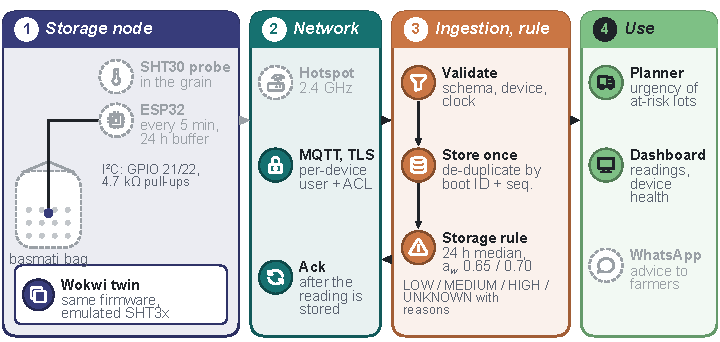
\includegraphics[width=\textwidth]{fig3_hardware.pdf}
  \caption{Storage node and data path. The ESP32 reads the probe in the grain (1) and sends each reading over MQTT with TLS (2); the
  server validates it, stores it once and applies the storage rule (3); and the planner and the manager app use the result (4). The
  firmware runs on a Wokwi twin~\cite{wokwi}; dashed grey parts (the physical probe, board and hotspot, and storage advice on
  WhatsApp) are the field deployment. ACL: access control list; I\textsuperscript{2}C: inter-integrated circuit bus; GPIO:
  general-purpose input/output.}
  \label{fig:node}
\end{figure}


\subsection{Stage 3: Manager Review and Approval}
\label{sec:method-approval}

A proposed plan is stored unchanged. A manager may edit it; each edit becomes a new revision that is
accepted only if the independent validator finds no violation, and the system's proposal is never
rewritten. Approval requires the \emph{approve} permission and an explicit acknowledgement of every
warning, refers to one revision, and in one database transaction records the decision and reserves
the exact quantities in the stock ledger. The reservation cannot exceed free stock, approval cannot
be given twice, and two plans competing for one lot cannot both succeed; this was tested with parallel
requests on PostgreSQL. A plan can also be rejected with a coded reason, and an unused reservation is
released by a person.

\subsection{Stage 4: Telling the Farmers}
\label{sec:method-messages}

After approval, one message per farmer is built from a versioned template in the farmer's recorded
language (Punjabi, Hindi or English) and the approved facts only: farmer name, variety, quantity,
mandi and date, with no price and no promise. A message can be prepared only if the farmer is active,
has a phone number and has agreed to WhatsApp messages; otherwise it is blocked with the reason,
and the checks are repeated at the moment of sending. A \emph{preview} channel shows the exact text
and a masked recipient without sending anything. For use without a messaging-platform account, the
manager can instead press ``Send to farmers'', confirm with yes or no, and receive one link per farmer
that opens the manager's own WhatsApp with the stored text already written; he sends it there and
reports ``sent'' or ``not sent'' for each farmer. The system cannot see delivery, so that report is
stored as the manager's statement and never as a delivery. Phone numbers are masked for every role
that may not see them, and each number shown is logged.

\subsection{Stage 5: Replies and Actual Sales}
\label{sec:method-sales}

Staff enter farmers' replies as text; a reply is stored and shown but never read as acceptance. A sale
is entered from the paper sale form (J-form) with lot, mandi, date, exact quantity and price; the amount
is computed exactly with ties to even, a duplicate form number is refused, and a mistaken entry is
voided by a compensating record. A sale on plan consumes its reserved stock; a sale off plan needs the
person to choose which reservation to give up (a provisional rule, not yet validated with an FPO). The
system then reports planned against actual quantity, price and share per farmer, and keeps forecast
outcomes of fictional and real sales apart.
